%====================================================================%
%                  MORIOND.TEX                                       %
%====================================================================%

\documentclass{moriond}

%\usepackage{lineno}
%\linenumbers

\bibliographystyle{unsrt}    
% for BibTeX - sorted numerical labels by order of
% first citation.

% A useful Journal macro
\def\Journal#1#2#3#4{{#1} {\bf #2}, #3 (#4)}

% Some useful journal names
\def\NCA{\em Nuovo Cimento}
\def\NIM{\em Nucl. Instrum. Methods}
\def\NIMA{{\em Nucl. Instrum. Methods} A}
\def\NPB{{\em Nucl. Phys.} B}
\def\PLB{{\em Phys. Lett.}  B}
\def\PRL{\em Phys. Rev. Lett.}
\def\PRD{{\em Phys. Rev.} D}
\def\ZPC{{\em Z. Phys.} C}
\def\JINST{\em Journ. of Instrum.}
\def\JHEP{\em Journ. of High Energy Phys.}
\def\PREP{\em Phys. Rep.}

% Some other macros used in the sample text
\def\st{\scriptstyle}
\def\sst{\scriptscriptstyle}
\def\mco{\multicolumn}
\def\epp{\epsilon^{\prime}}
\def\vep{\varepsilon}
\def\ra{\rightarrow}
\def\ppg{\pi^+\pi^-\gamma}
\def\vp{{\bf p}}
\def\ko{K^0}
\def\kb{\bar{K^0}}
\def\al{\alpha}
\def\ab{\bar{\alpha}}
\def\be{\begin{equation}}
\def\ee{\end{equation}}
\def\bea{\begin{eqnarray}}
\def\eea{\end{eqnarray}}
\def\CPbar{\hbox{{\rm CP}\hskip-1.80em{/}}}
%temp replacement due to no font
%%%%%%%%%%%%%%%%%%%%%%%%%%%%%%%%%%%%%%%%%%%%%%%%%%
%                                                %
%    BEGINNING OF TEXT                           %
%                                                %
%%%%%%%%%%%%%%%%%%%%%%%%%%%%%%%%%%%%%%%%%%%%%%%%%%

%\newcommand{\Photo}{\includegraphics[height=35mm]{mypicture}}
\newcommand{\Photo}{}

\begin{document}
\vspace*{4cm}
\title{Exotic searches by CMS}

\author{Francesco Santanastasio}

\address{Sapienza, Universit\`a di Roma ed INFN Sezione di Roma on
  behalf of the CMS Collaboration}

\maketitle\abstracts{
These proceedings present the results of new searches for various new
physics phenomena in proton-proton collisions at $\sqrt{s}=13$~TeV and $13.6$~TeV
delivered by the LHC and collected with the CMS detector during Run 2
(2016-2018) and Run 3 (2022-2023), respectively. In many cases these analyses
set the most stringent limits on these new physics phenomena to date. 
}

\section{Introduction}

These proceedings present the results of searches for various new physics phenomena beyond the standard model (SM) in proton-proton
collisions delivered by the LHC and collected with the Compact Muon Solenoid (CMS)~\cite{CMS:2008xjf,CMS:2023gfb}
detector. The focus will be on results from the Exotica (EXO) working
group, looking for exotic new physics signatures. For the majority of these searches the full Run 2
(2016-2018) dataset has been used, corresponding to an integrated
luminosity of about 140~fb$^{-1}$ at  $\sqrt{s}=13$~TeV. Some new results with early Run 3
data collected in 2022 (with a total integrated luminosity of
about 35~fb$^{-1}$ at  $\sqrt{s}=13.6$~TeV) are also shown in Section~\ref{sec:run3}.
A choice was made by the author to show only recent results, most of
them never presented before at a major conference, and to avoid overlaps with
other reports including CMS material during the same conference. The
report covers a few important aspects which are relevant nowadays
in the design of EXO searches: follow up on excesses of events
observed in data; explore new experimental signatures and final states;
developments in trigger and analysis methods. Limits on parameters of
theory models or resonance masses will be provided at 95\% confidence level
(CL). The updated lists of published results,
preliminary results and summary plots from the EXO group are reported at Refs.~\cite{CMS:EXOpub,CMS:EXOprel,CMS:EXOsum}.

\section{New heavy resonances}

A search for new physics in high-mass diphoton events~\cite{CMS-PAS-EXO-22-024}
($m_{\gamma\gamma}>500$~GeV) was performed to look for either
a bump (search for new resonances) or a broad deviation (non-resonant search) in the
diphoton mass spectrum compared to what predicted by SM background processes.
In the search for resonant excesses from both the spin-2
Randall-Sundrum (RS) and spin-0 heavy Higgs boson models, the diphoton mass spectrum is fit to a
parameterized functional form, allowing for a description of the background shape
based exclusively on data. Different resonance widths are probed
($10^{-4}$, 1\%, 5\%).
In the search for non-resonant excesses that arise from the ADD extra dimension and clockwork models, a
next-to-next-to-leading order (NNLO)
calculation in quantum chromodynamics (QCD) is employed to estimate
the SM diphoton background. The largest excess seen in the
resonant search is at a resonance mass of about 1.3 TeV corresponding to a
significance of 2.6 standard deviation ($\sigma$) local, and
0.8$\sigma$ global after accounting for the lookelsewhere effect. No
excess is observed by the corresponding ATLAS analysis. The CMS
analysis excludes the existence of RS gravitons (with model parameter
$\tilde{k}=0.1$) with masses below 4850~GeV at 95\% CL, compared to 4500~GeV of
ATLAS. No significant deviation is observed in the non-resonant search
and limits are set on the ADD model (lower limits on mass scale $M_S$
ranging from 7.1 to 11.1~TeV depending on the specific theoretical convention) and
clockwork model (with the fundamental scale $M_5$ excluded below
8.0 TeV for spring parameter $k$ values between 0.2 GeV and 2.0 TeV) providing comparable
sensitivity to ATLAS.

A search for new spin-0, charged resonance decaying to a W boson and a photon
was performed~\cite{CMS-PAS-EXO-21-017}, considering leptonic W decays in electron and muon
final states with sizeable missing transverse energy (MET) coming from
neutrinos. The analysis consists in looking for a bump in the
transverse mass spectrum, built from the reconstructed charged lepton
and the MET. No significant excess is observed in data under the
hypothesis of either a narrow (0.01\%) or a broad (5\%) relative width
for the new resonance. The results of the leptonic channel are combined with an existing CMS search for
the same resonance in the complementary final state with hadronic W
decays (jets). After the combination, the largest local excess is at
1.6~TeV mass with a local significance of 2.7$\sigma$ (2.5$\sigma$) for the
narrow (broad) resonance scenario. The combined analysis provides the most
stringent limits to date in the 0.3-2~TeV mass range.

A more exotic experimental signature was considered in a new search
for a massive resonance $X$ decaying to a pair of spin-0
bosons $\phi$ that themselves decay to pairs of photons~\cite{CMS:2024vjn}.
The analysis probes resonance masses $m_X$ between 0.3 and 3~TeV,
and is restricted to values of $m_{\phi}$ for which the ratio
$\alpha=\frac{m_{\phi}}{m_X}$ is between 0.5\% and 2.5\%. For these
values of $\alpha$, the two photons (diphoton) from each $\phi$ boson
are expected to be very close in space, generating energy deposits
in the electromagnetic calorimeter (ECAL) detector with a significant
spatial overlap.  Each pair of photons from $\phi$ decay is reconstructed
as a single cluster in ECAL ($\Gamma$) with a prominent dipolar
substructure. Neural networks are designed to classify events containing
such diphotons and to reconstruct the mass of the diphoton object ($m_{\Gamma}$)
using the shapes of energy deposits in ECAL. 
The invariant mass spectra of $\Gamma\Gamma$ candidates are
analyzed for the presence of the $X$ resonance, in different bins of
the reconstructed $\alpha^{reco}$ variable, defined as the ratio between the
average cluster mass $<m_{\Gamma}>$ and the di-cluster invariant mass $m_{\Gamma\Gamma}$,
in order to be sensitive to a wide range of different $X$ and $\phi$ mass
hypotheses. The largest excess in data compared to background
predictions is observed for $m_X \sim 720$~GeV and $m_{\phi} \sim 6$~GeV
corresponding to a local (global) significance of $3.6\sigma$
($1\sigma$). This is currently the most sensitive search at the LHC in this
final state.

\section{Physics of dark sector}

The so-called Hidden Valley models of new physics beyond SM consider a
``dark sector'' that extends the SM with a non-Abelian gauge group,
similar to QCD, with new matter and gauge
fields analogous to the SM quark and gluon fields. The SM particles
are neutral under the new, dark interaction — “dark QCD” — and
communicate with this sector only through a mediator particle that
couples to both sectors. Depending on the model parameters, the
formation process of jets in dark QCD showers (including fragmentation,
hadronization and decays) can result in very different experimental
signatures compared to the SM QCD. In this report, two different
scenarios were considered.

The first search~\cite{CMS:2024nca} considers the process $pp \rightarrow S \rightarrow \chi
\chi$ were $S$ is the mediator between SM and dark sector and $\chi$
is a quark of the dark sector (dark quark). While high momentum SM quarks
produce collimated sprays of particles (jets), in this model a dark
quark from the decay of an $S$ particle produced at rest, generates a characteristic final state consisting of many
low-momentum, isotropically distributed particles —  described
as a soft unclustered energy pattern (SUEP) — which would be very
difficult to trigger. The analysis strategy employed high momentum ($p_T$) jet triggers to
select events where the scalar mediator $S$ is produced with large
Lorentz-boost recoiling against an initial-state radiation (ISR)
jet. The $S$ decay products are collected within a wide-cone jet (SUEP-jet) with
a peculiar internal substructure. The energy pattern inside a SUEP-jet shows in fact
a characteristic isotropic shape and a large multiplicity of particles, as shown in Fig.~\ref{fig:darksector}. The number of tracks and the associated sphericity
observable in the SUEP-jet candidate are used to discriminate between the signal and the
background, which is estimated from data in suitable control regions.
With no observed excess of events over the SM expectation,
limits are set on the model parameters. This result represents the first dedicated
search for SUEPs at LHC.

The second search~\cite{CMS:2024gxp} focuses on the pair production
process $pp \rightarrow \phi\phi$ where each dark sector mediator $\phi$ decays to a SM
quark and a dark quark. In this scenario, the dark quark showers and
hadronizes, it produces long-lived dark mesons (with a characteristic
lifetime $\tau_{dark}$) that subsequently decay into SM particles, resulting in a jet
— known as an emerging jet (EJ) — with multiple displaced
vertices. A graph neural network (GNN), which takes in input several reconstructed
observables (eg. the transverse impact parameter of tracks in a jet), is used to discriminate between the
signal EJ and background QCD jets. In addition, a more model
agnostic search based on a traditional cut-based selection is also
performed. No excess of events beyond the SM expectations is found and
upper limits are set on the production cross section as a function of the mediator mass and $c\tau$, for different
hypotheses on the dark meson mass. The CMS experiment covers a wide
range of $c\tau_{dark}$ values for this benchmark model (from 1~mm to
$10^2$~m) exploiting both the EJ search and a complementary search
based on muon detector showers, as shown in Fig.~\ref{fig:darksector}.

\begin{figure}
\begin{minipage}{0.33\linewidth}
\centerline{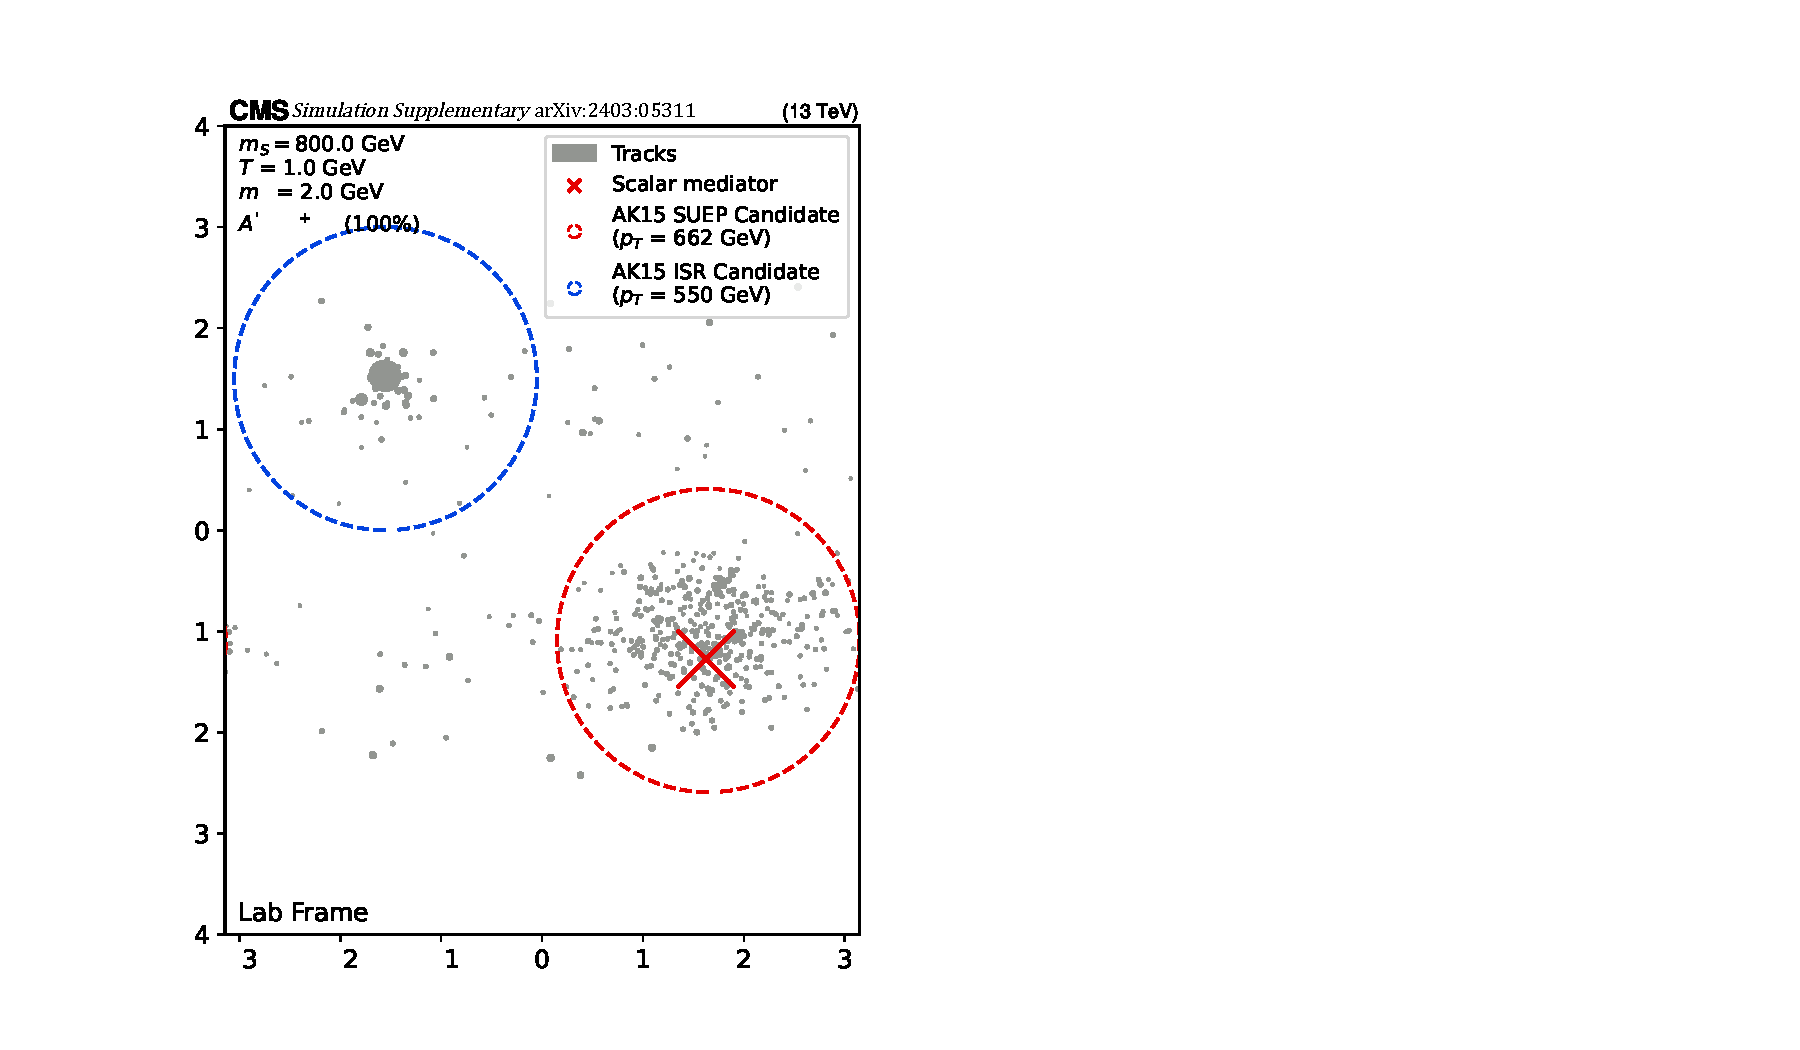
\includegraphics[width=1.0\linewidth]{CMS-EXO-23-002_Figure-aux_005.pdf}}
\end{minipage}
\hfill
\begin{minipage}{0.65\linewidth}
\centerline{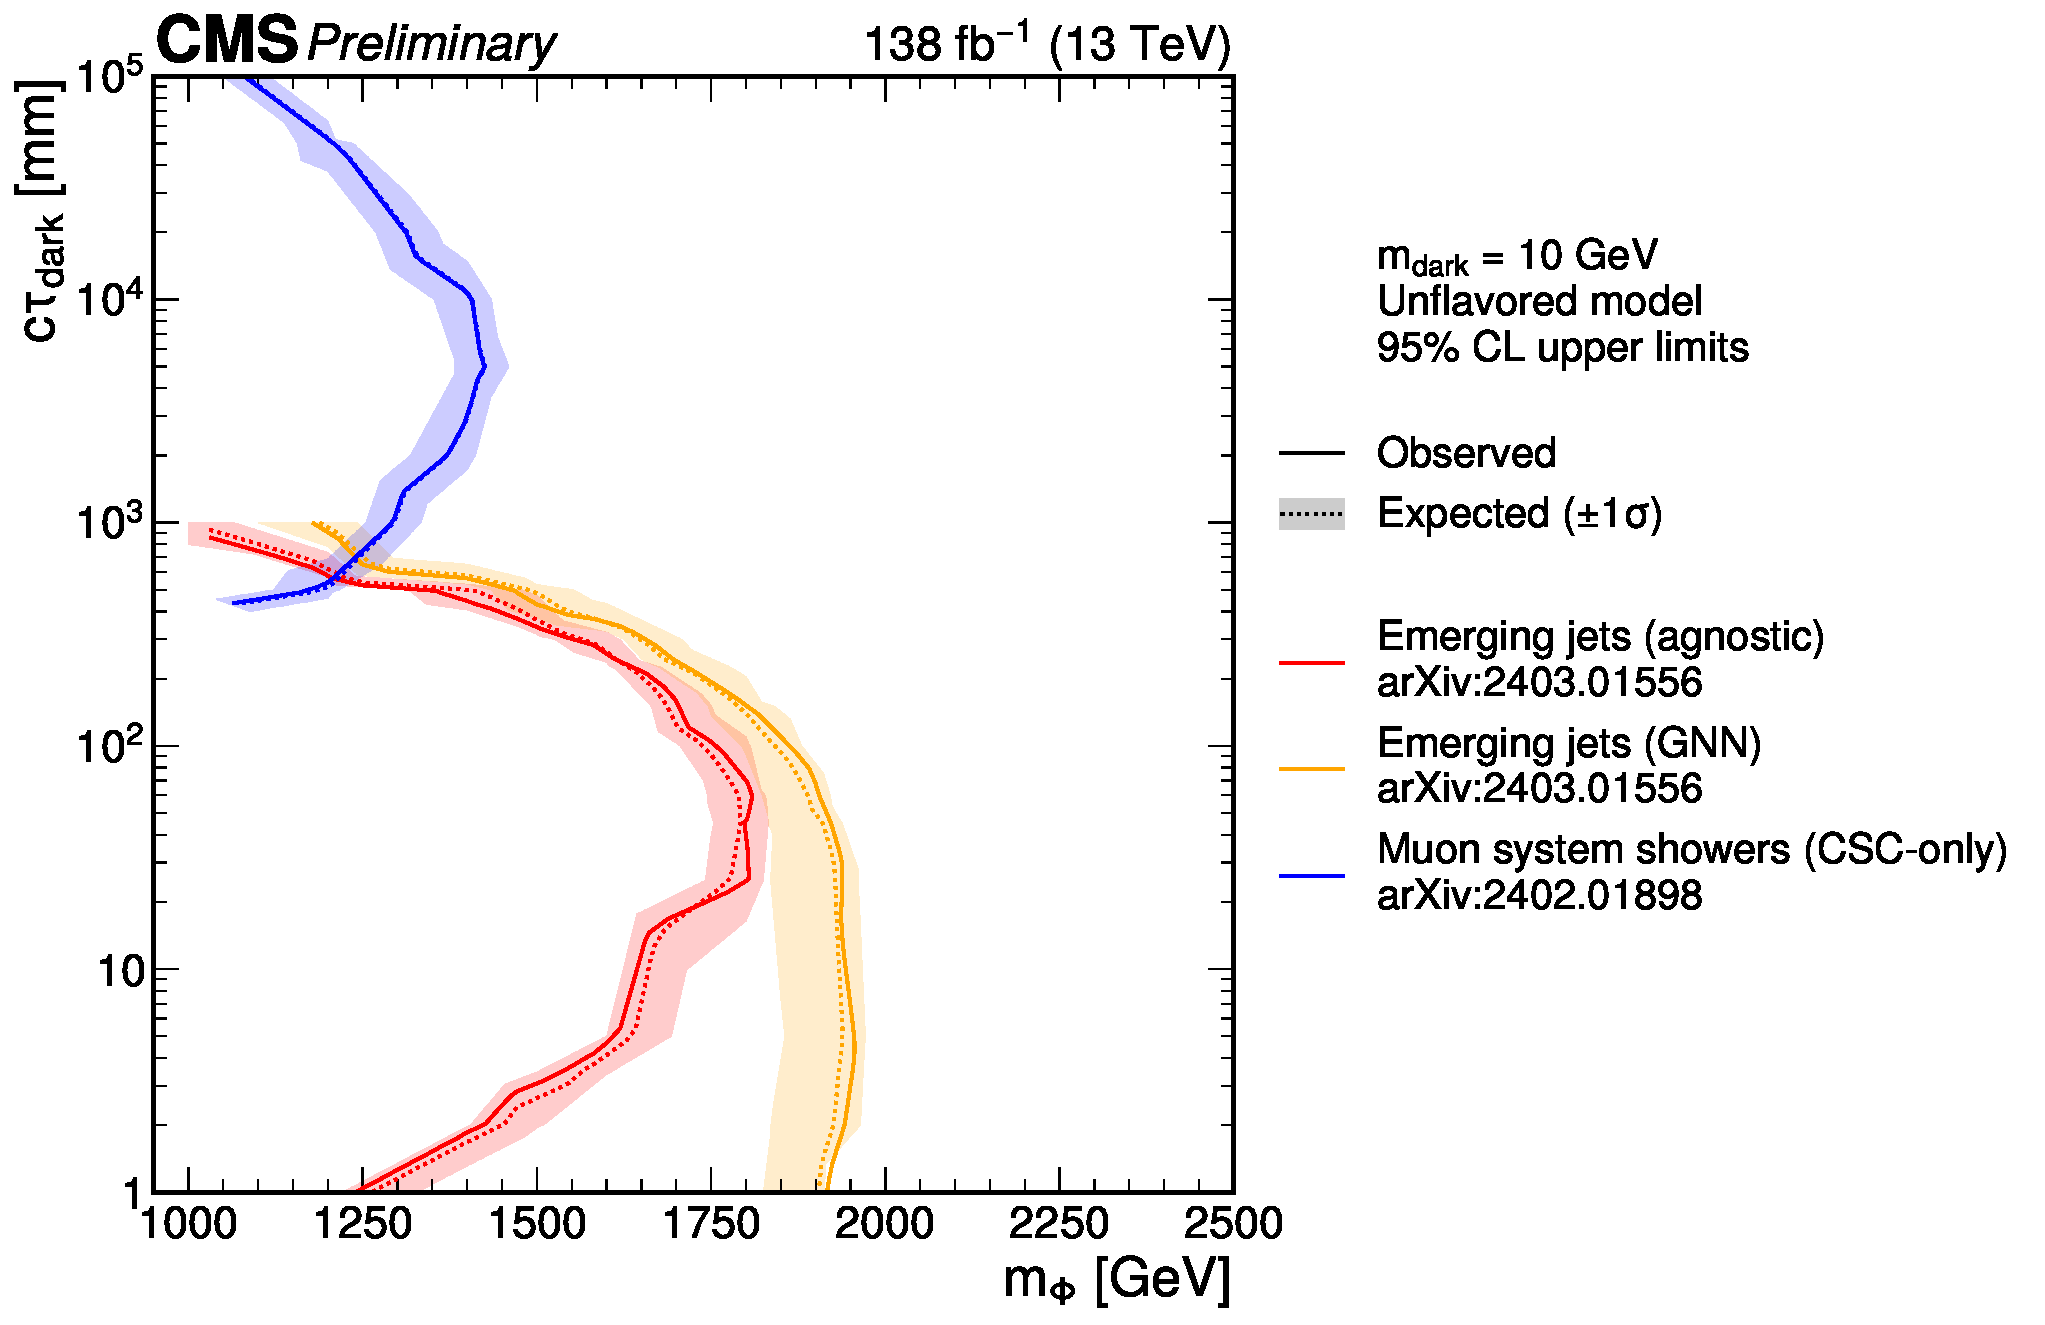
\includegraphics[width=1.0\linewidth]{emj_EXO-22-015_EXO-21-008_limits_unflavored_prelim.pdf}}
\end{minipage}
\caption[]{An example signal event from a representative SUEP model
  with a resonance mass of 800 GeV, taken from Ref.~\cite{CMS:2024nca} (left). Exclusion limits from the
  track-based and muon detector shower-based searches for pair
  production of a mediator particle $\phi$ that decays to a jet and an
  emerging jet, taken from Ref.~\cite{CMS:2024gxp} (right).}
\label{fig:darksector}
\end{figure}

\section{Data scouting}

Theories beyond the SM often leads to the prediction of new light
particles with feeble couplings. These events may not be collected in
pp collisions due to high energy thresholds in standard triggers. Specialized data-taking and
data-processing strategies were introduced by the CMS experiment in
Run 1 (2010-2012) of the CERN LHC to enhance the sensitivity to such
particles. The novel data-scouting strategy (first introduced at the end of 2011) enhances sensitivity to
low-energy physics processes by significantly lowering the high-level
trigger (HLT) thresholds and storing a reduced event content on disk,
as shown schematically in Fig.~\ref{fig:scouting}.
For events passing these loose trigger selections, only high-level physics
objects (such as charged leptons or jets) reconstructed at the HLT are stored
on disk, with no raw data from detector channels. These dedicated data
samples are then used offline to perform physics analysis. The CMS experiment has greatly expanded the sensitivity to
resonances with low mass $m_X$ thanks to data scouting, for both final
states with dijets/multijets ($50<m_X<1500$~GeV) and dimuons ($2m_{\mu}<m_X<40$~GeV).
CMS has released for this conference a review paper~\cite{CMS:2024zhe}
on this topic which describes the origin and evolution of data scouting in CMS, including
performance studies of HLT reconstructed objects and results of physics measurements.

The data scouting was significantly improved for the ongoing Run 3. A factor 4
increase in scouting HLT rate compared to Run 2 (up to a max. of 30
kHz) was reached. This improvement was made possible thanks to a new fast tracking based on pixel-detector
only (``Patatrack'' algorithm) and the use of graphical user interfaces (GPUs) at HLT.
A single data-scouting stream is now collected with full event record
of Particle Flow (PF). The PF is algorithm that aims to reconstruct and
identify each individual particle (called a PF candidate) in a pp collision event,
with an optimized combination of information from the various elements
of the CMS detector. The event content is still reduced but rich enough to
perform complex offline analyses, and it includes PF candidates, jets, muons,
electrons, photons, tracks, and vertices reconstructed at HLT. The
presence of PF candidates makes possible, for example, to perform offline
the reclustering of jets and to study the jet substructure.

A prime example of the discovery potential with the data scouting
approach is represented by the CMS search for multijet resonances. This is a
comprehensive analysis that looks for pair produced resonances each
decaying into two or three jets in both boosted and resolved final
states. The focus of the conference report was on the resolved 6-jet
final state. The corresponding benchmark signal model is the pair production of a pair
of gluinos each decaying to three quarks, as foreseen in Supersymmetry models
with R-parity violation (RPV SUSY). The search looks for a bump in the trijet
mass spectrum after a set of selection criteria that reduce the SM QCD
background and enhance the specific signal topology. The largest local
excess is observed at a resonance mass of about 770 GeV with a local significance of
2.6$\sigma$. Figure~\ref{fig:scouting} shows that the
upper limits on signal cross section are a factor 10 to 100 times more
stringent in the sub-TeV mass range than other experiments (which use instead a
traditional trigger strategy) and probe resonances masses as low as 70
GeV, thanks to the data-scouting approach.

\begin{figure}
\begin{minipage}{1.0\linewidth}
\centerline{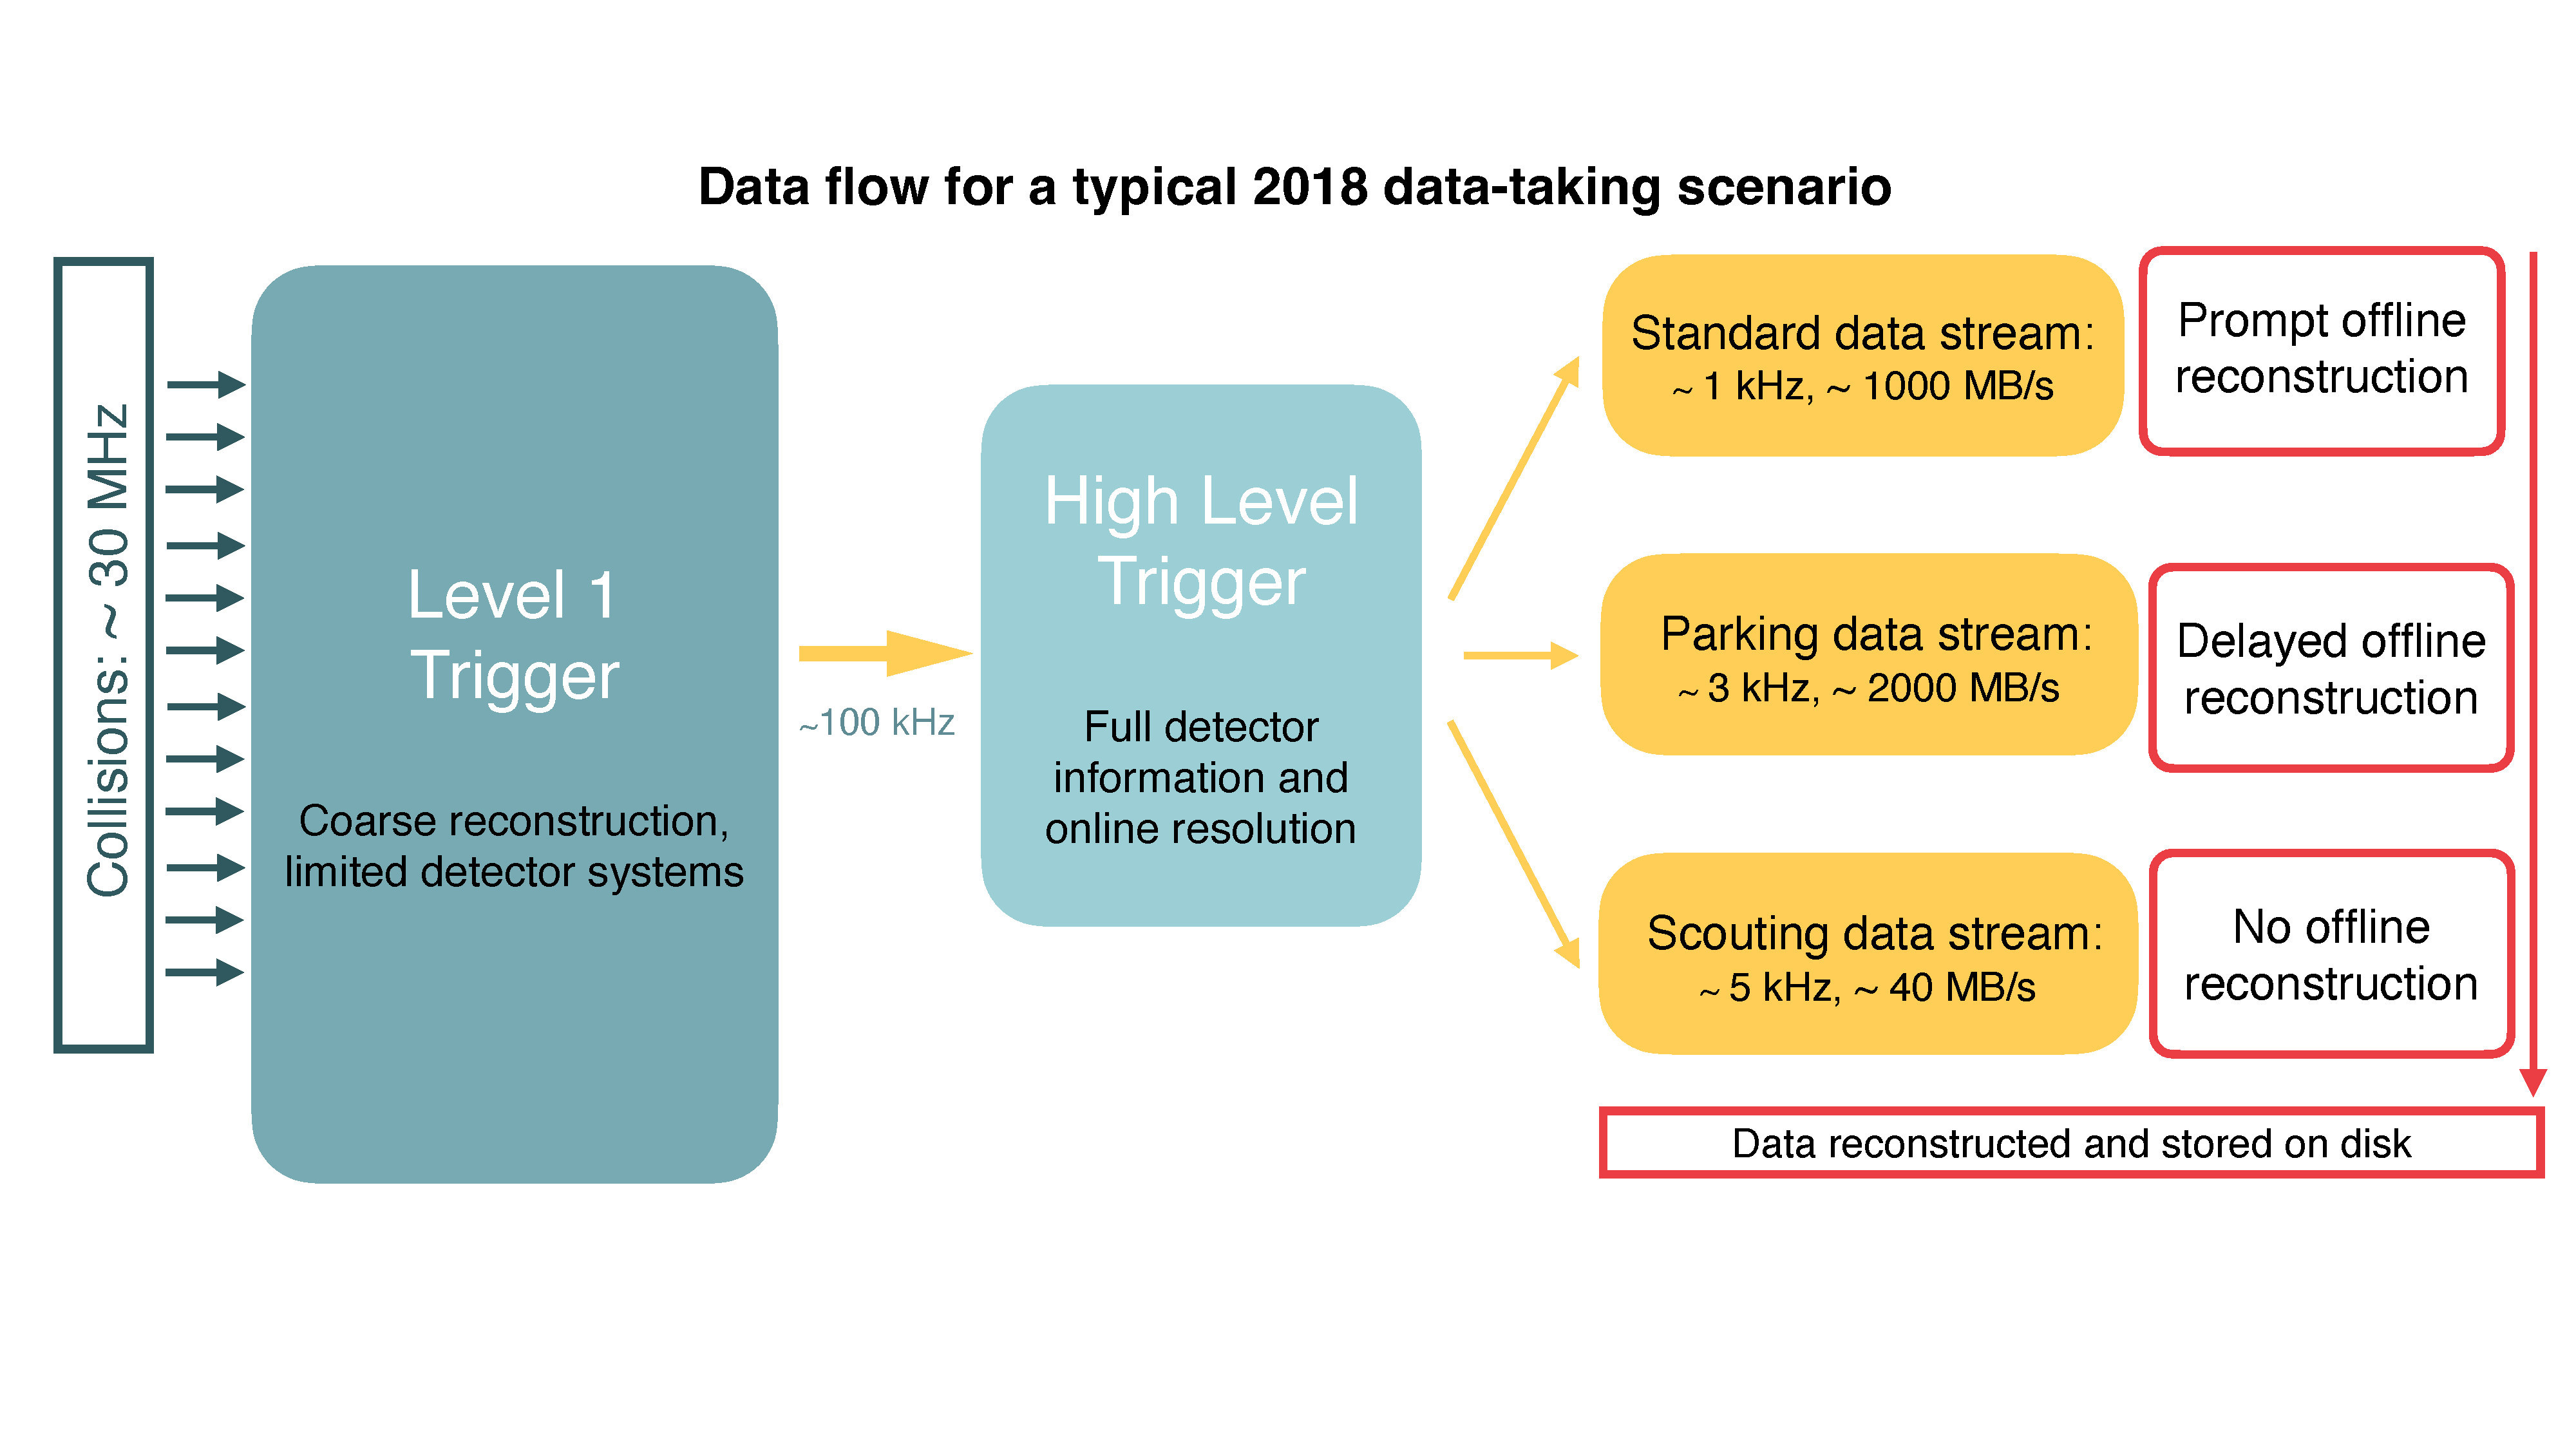
\includegraphics[width=0.7\linewidth]{CMS-EXO-23-007_Figure_001.pdf}}
\end{minipage}
\hfill
\begin{minipage}{1.0\linewidth}
\centerline{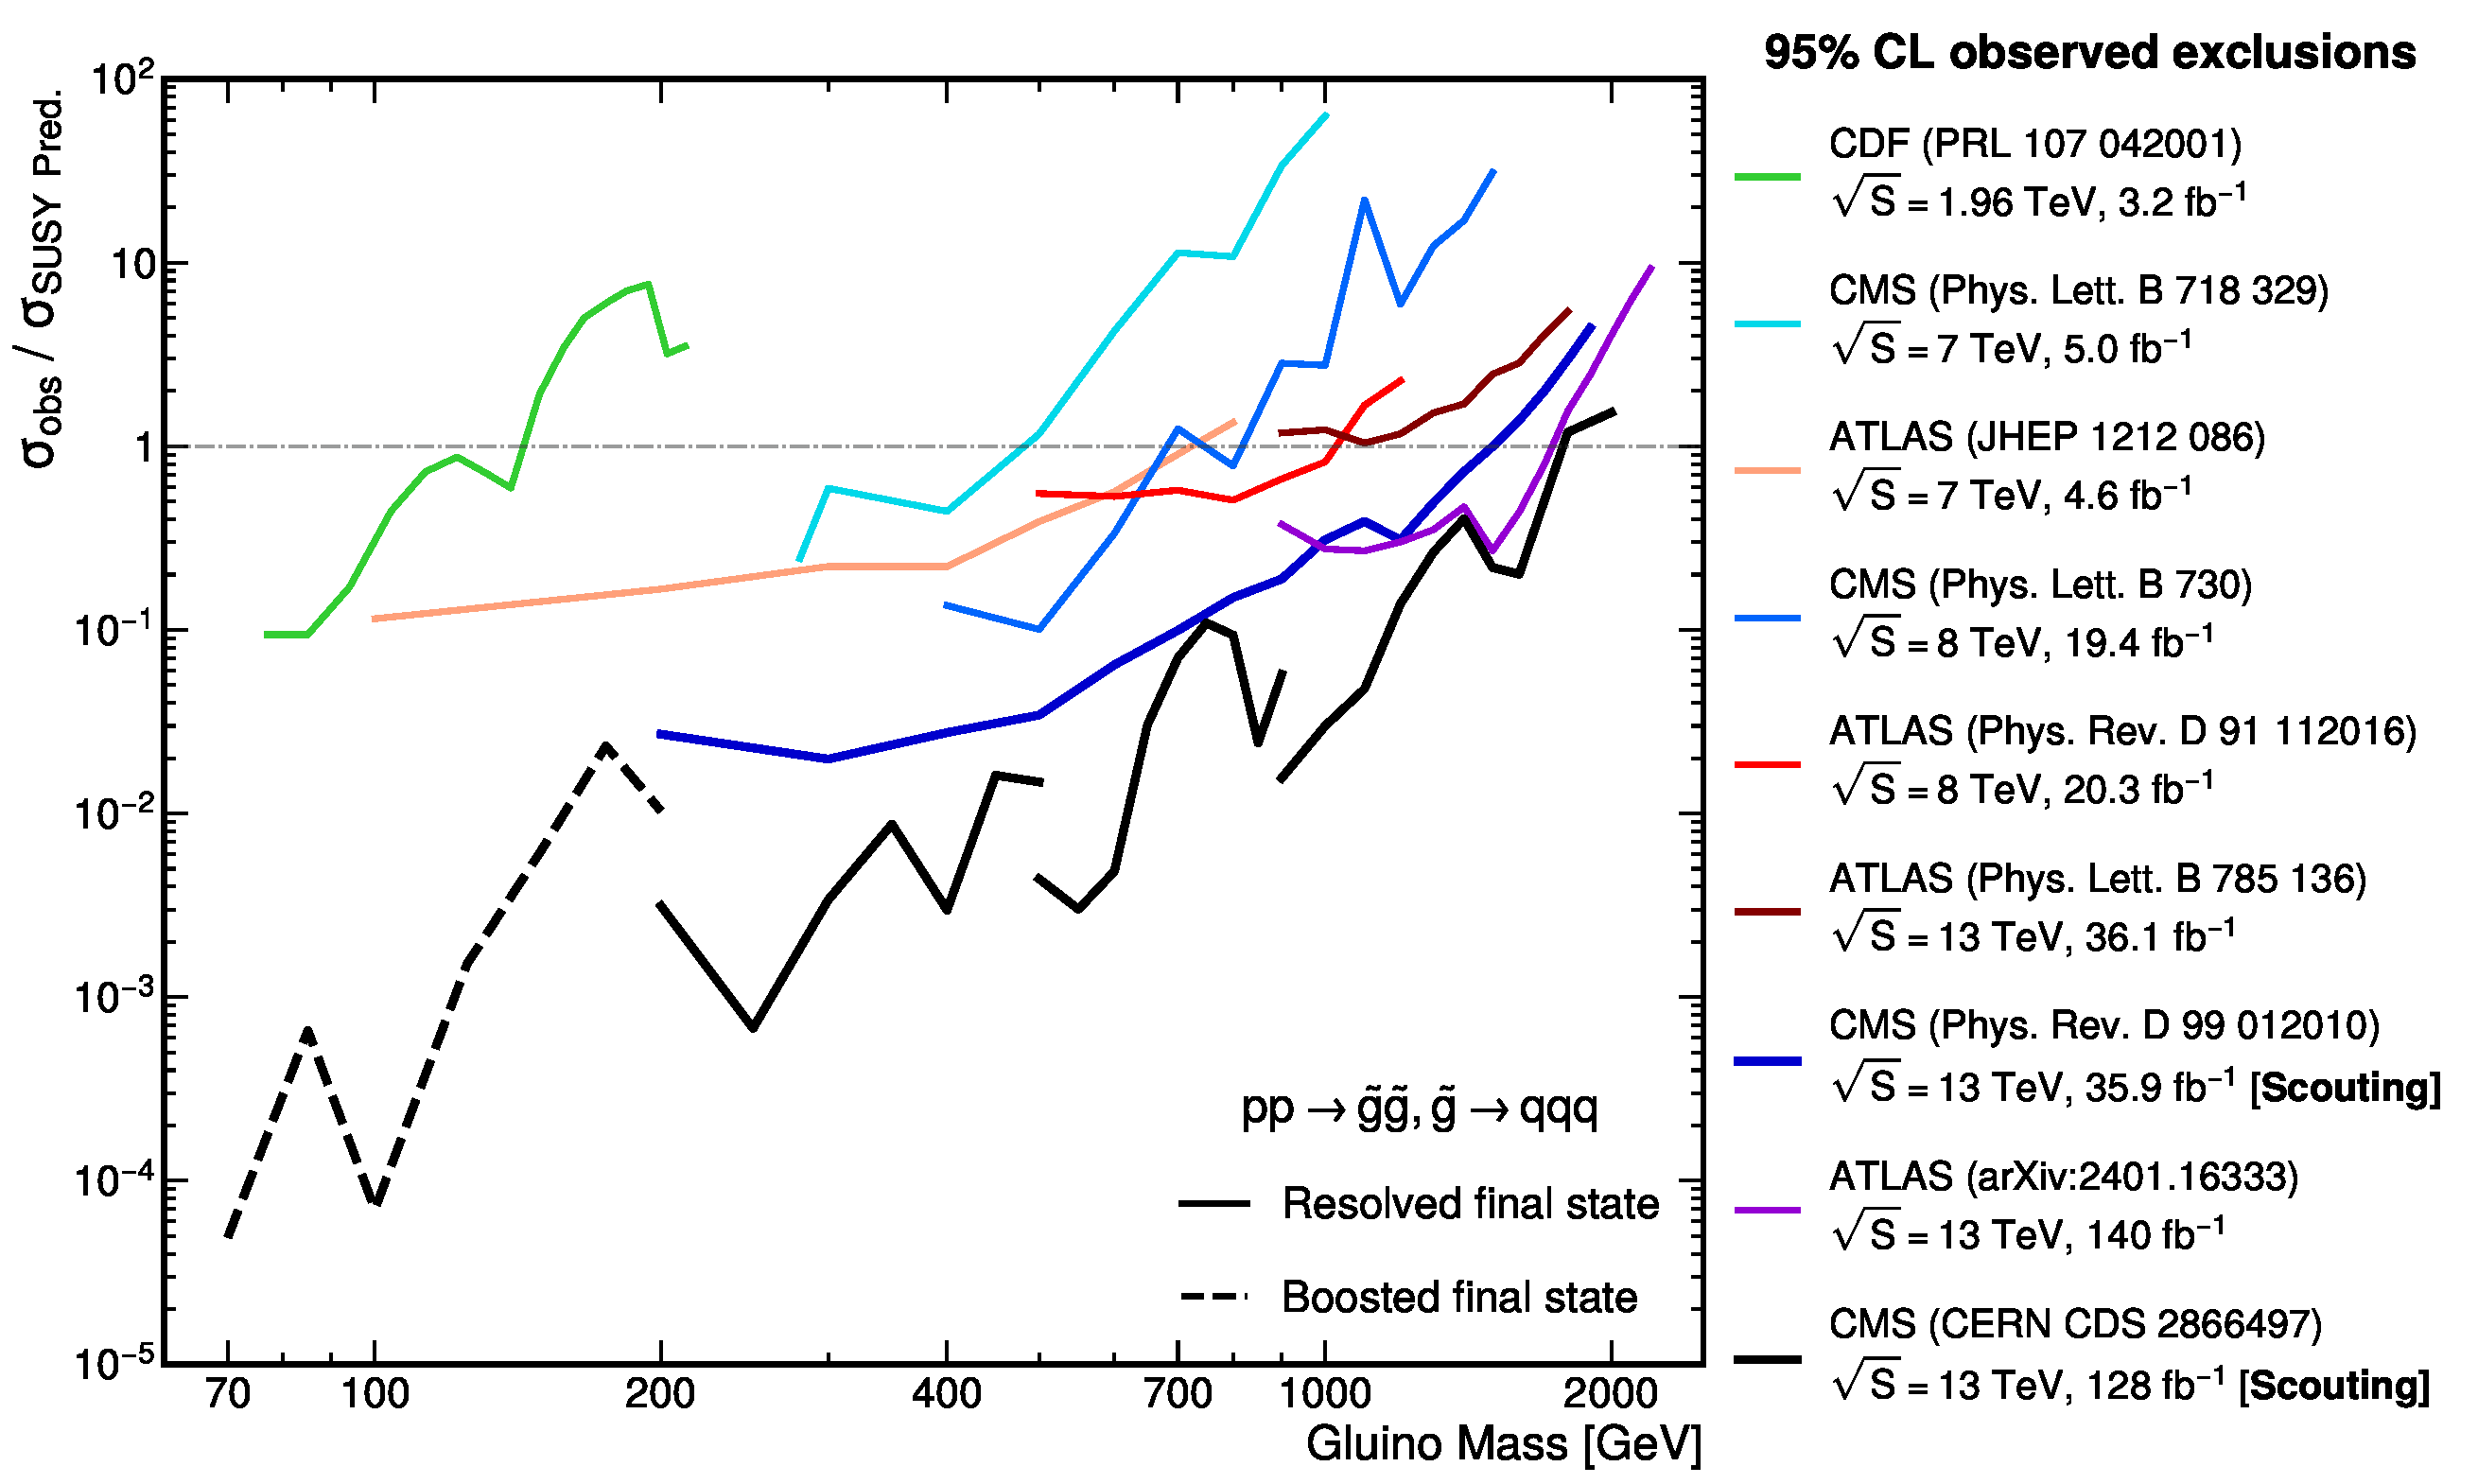
\includegraphics[width=0.7\linewidth]{CMS-EXO-23-007_Figure_016.pdf}}
\end{minipage}
\caption[]{A schematic view of the typical Run 2 data flow during 2018
  showing the data acquisition strategy with scouting and parking data
  streams, along with the standard data stream (left). Comparison of
  limits from searches for RPV gluinos decaying to three partons
  (right). Plots taken from Ref.~\cite{CMS:2024zhe}.}
\label{fig:scouting}
\end{figure}


\section{New Run 3 results} \label{sec:run3}

A new search for low-mass long-lived particles (LLPs) decaying to displaced
jets~\cite{CMS-PAS-EXO-23-013} was presented during this conference.
The benchmark signature for this search is the exotic decay of the 125
GeV Higgs boson ($H$) to two long-lived neutral scalars $S$ ($H
\rightarrow SS$), each of which further decays to a pair of SM fermions (bb, dd, or $\tau\tau$
hadronic final states were considered).  The target signature is a pair of jets, referred to as a
dijet, arising from the decay of the LLP. Displaced vertices (DVs) can be reconstructed using
the displaced tracks associated with the dijet. The properties of the tracks, DVs, and dijet are
used to discriminate between exotic LLP signatures and SM background
processes. Major improvements compared to the previous CMS analysis
were introduced: new triggers~\cite{CMS-DP-2023-043} (increasing the signal acceptance by a
factor 10 compared to Run 2); a new reconstruction for
displaced secondary and tertiary vertices (the latter coming mainly
from in flight decays of B mesons to D mesons); a new LLP tagging
based on GNNs. No excess was observed in data. Upper limits were set
on the branching fraction of the $H \rightarrow SS$ decay as a function
of the proper decay length $c\tau_{0}$ of the LLP. These are the best limits to date for LLPs
in the 15-55~GeV mass range and with $c\tau_{0}<1$~m.
The sensitivity of this CMS analysis based on Run 3 data is up to 10 times better (in terms
of upper limits on branching fraction) than a similar ATLAS Run 2 search
despite the 4 times smaller dataset, thanks to both trigger and analysis improvements.

\begin{figure}
\begin{minipage}{0.5\linewidth}
\centerline{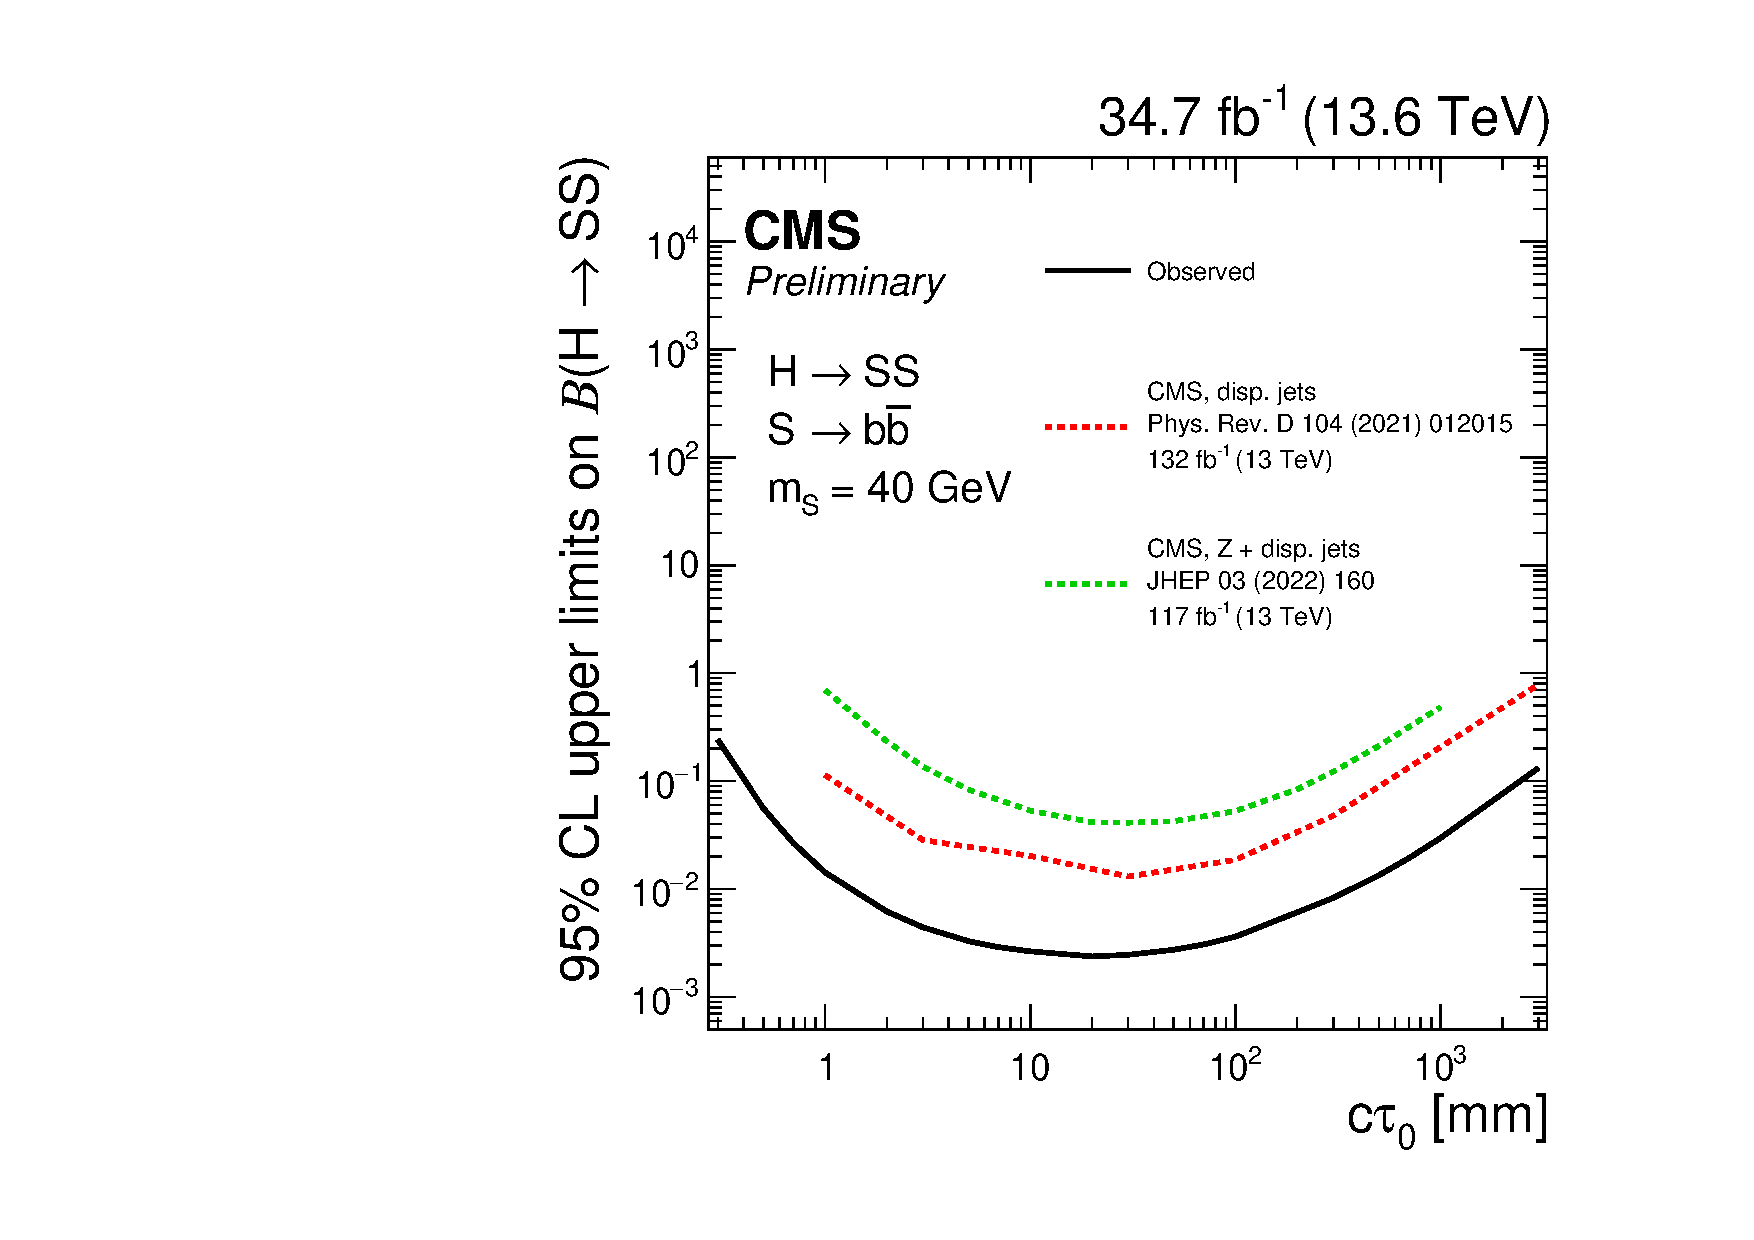
\includegraphics[width=1.0\linewidth]{CMS-PAS-EXO-23-013_Figure_004-a.pdf}}
\end{minipage}
\hfill
\begin{minipage}{0.5\linewidth}
\centerline{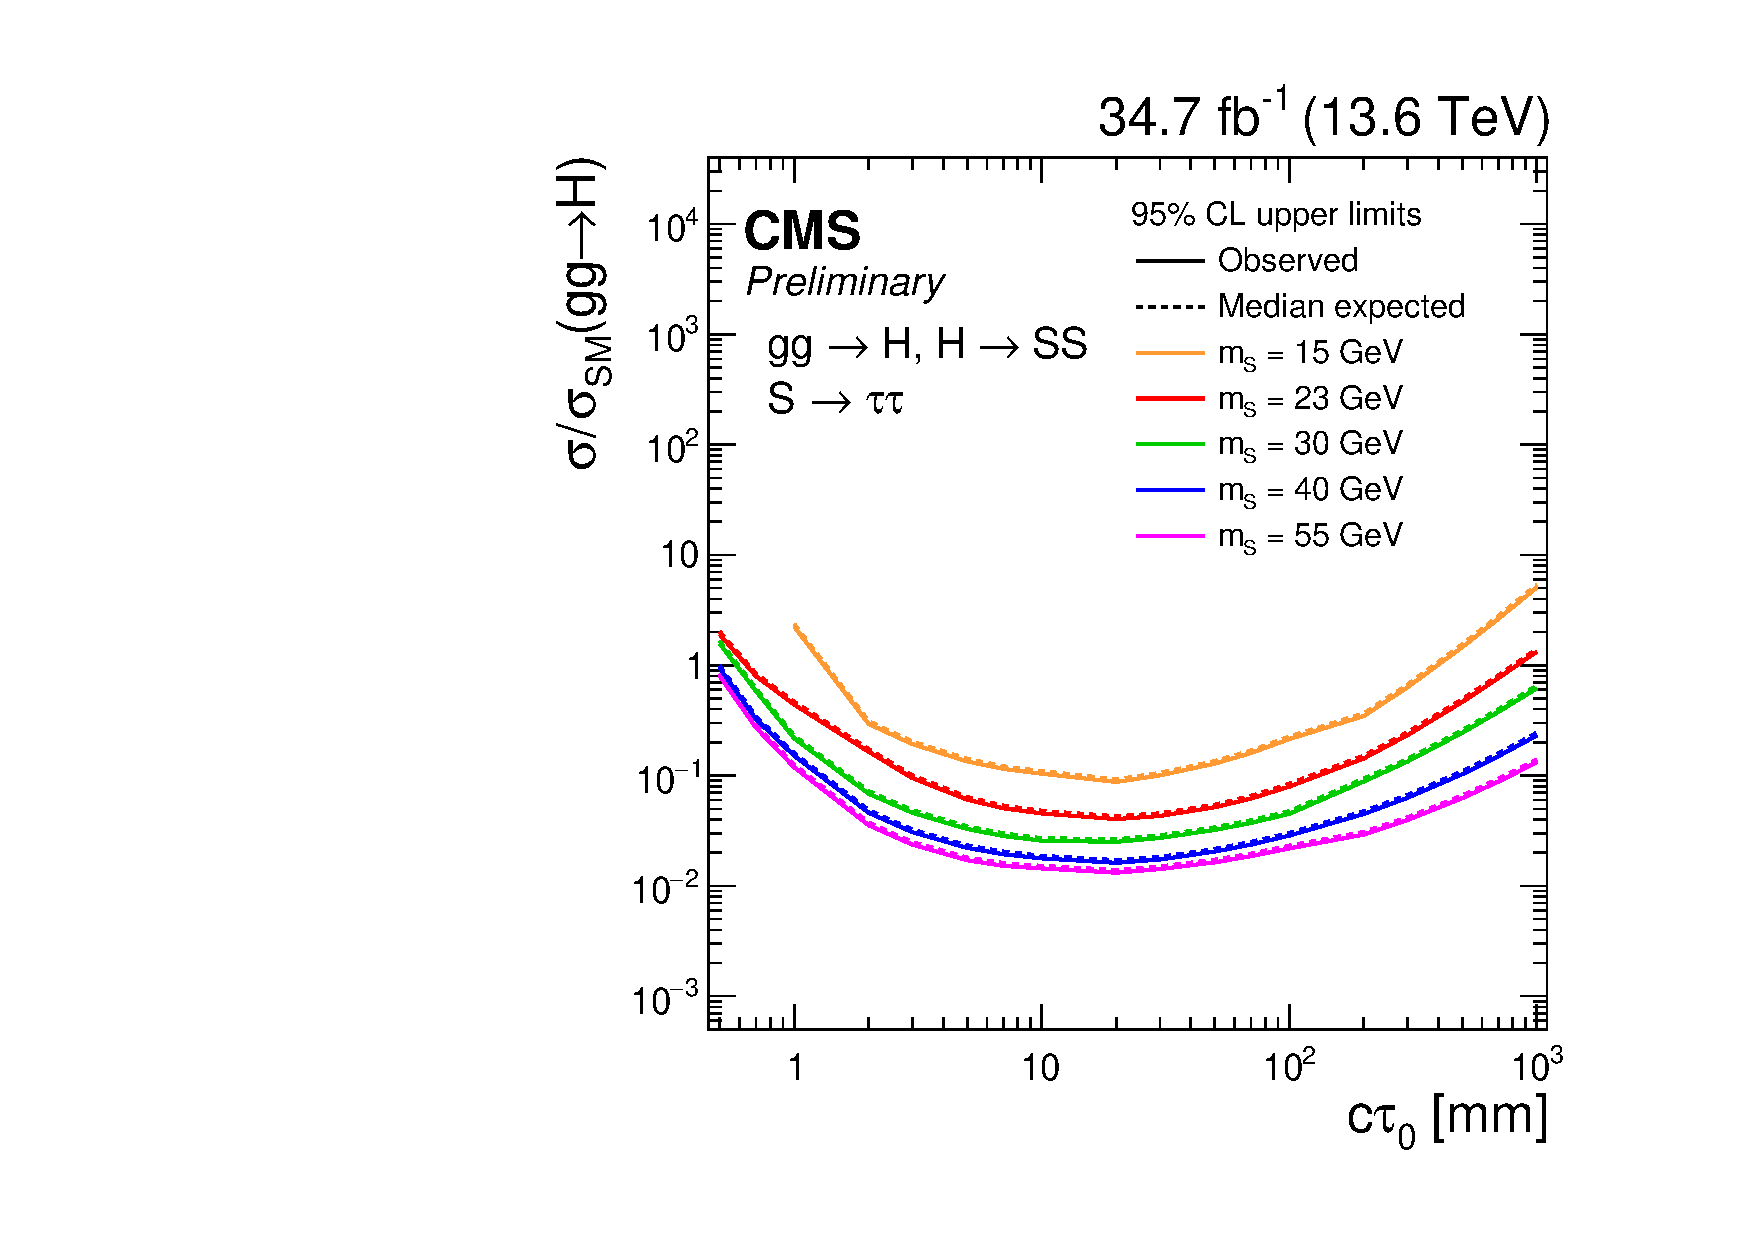
\includegraphics[width=1.0\linewidth]{CMS-PAS-EXO-23-013_Figure_003-c.pdf}}
\end{minipage}
\caption[]{Upper limits on the branching fraction of the $H \rightarrow
  SS$ decay for $S\rightarrow bb$ (left) and $S\rightarrow \tau\tau$
  (right) for different LLP masses $m_S$ and proper decay lengths
  $c\tau_{0}$. These are the first limits for the $S \rightarrow
  \tau\tau$ decay. Plots taken from Ref.~\cite{CMS-PAS-EXO-23-013}.}
\label{fig:run3}
\end{figure}

\section*{Acknowledgments}

The author wishes to thank the organizers of the “Rencontres de
Moriond/EW” for the rich and interesting physics program, and the
beautiful location of the conference. Thank you for creating the usual
relaxed and confidential atmosphere which made interesting discussions
possible among the participants.

\section*{References}

\begin{thebibliography}{99}

\bibitem{CMS:2008xjf} The CMS Collaboration, \Journal{\JINST}{3}{S08004}{2008}.
\bibitem{CMS:2023gfb} The CMS Collaboration, \Journal{Submitted to \JINST}{}{arXiv:2309.05466}{2023}.
\bibitem{CMS:EXOpub} The CMS Collaboration, EXO published results,
  \url{https://cms-results.web.cern.ch/cms-results/public-results/publications/EXO/index.html}.
\bibitem{CMS:EXOprel} The CMS Collaboration, EXO preliminary results,
  \url{https://cms-results.web.cern.ch/cms-results/public-results/preliminary-results/EXO/index.html}.
\bibitem{CMS:EXOsum} The CMS Collaboration, EXO summary plots,
  \url{https://twiki.cern.ch/twiki/bin/view/CMSPublic/SummaryPlotsEXO13TeV}.
\bibitem{CMS-PAS-EXO-22-024} The CMS Collaboration, \Journal{To be
    submitted for publication}{}{CMS-PAS-EXO-22-024 \url{https://cds.cern.ch/record/2893028}}{2024}.  
\bibitem{CMS-PAS-EXO-21-017} The CMS Collaboration, \Journal{To be
    submitted for publication}{}{CMS-PAS-EXO-21-017 \url{https://cds.cern.ch/record/2893032}}{2024}.  
\bibitem{CMS:2024vjn} The CMS Collaboration, \Journal{Submitted to \PRL}{}{arXiv:2405.00834}{2024}.
\bibitem{CMS:2024nca} The CMS Collaboration, \Journal{Submitted to
    \PRL}{}{arXiv:2403.05311}{2024}.
\bibitem{CMS:2024gxp} The CMS Collaboration, \Journal{Submitted to
    \JHEP}{}{arXiv:2403.01556}{2024}.
\bibitem{CMS:2024zhe} The CMS Collaboration, \Journal{To be submitted
    to \PREP}{}{arXiv:2403.16134}{2024}. 
\bibitem{CMS-PAS-EXO-23-013} The CMS Collaboration, \Journal{To be
    submitted for publication}{}{CMS-PAS-EXO-23-013 \url{https://cds.cern.ch/record/2893044}}{2024}. 
\bibitem{CMS-DP-2023-043} The CMS Collaboration, CMS-DP-2023-043
  \url{https://cds.cern.ch/record/2865844} (2023).

\end{thebibliography}

\end{document}

%%%%%%%%%%%%%%%%%%%%%%
% End of moriond.tex  %
%%%%%%%%%%%%%%%%%%%%%%


%%% Local Variables: 
%%% mode: latex
%%% TeX-master: t
%%% End: 

%%% Local Variables: 
%%% mode: latex
%%% TeX-master: t
%%% End: 

%%% Local Variables: 
%%% mode: latex
%%% TeX-master: t
%%% End: 
